\documentclass[11pt]{article}
%\documentclass{book}
\usepackage[utf8]{inputenc}
\usepackage[T1]{fontenc}
\usepackage[french]{babel}
\usepackage[top=1.8cm, bottom=1.8cm, left=1.8cm, right=1.8cm]{geometry}
\usepackage[linktocpage,colorlinks=false]{hyperref}
\usepackage{graphicx}
\usepackage{epsfig}
\usepackage{amssymb}
\usepackage{amsmath}
\usepackage{array}
\usepackage{subfig}
\usepackage{multicol}
\usepackage{caption}
\usepackage{listings}
\usepackage{algorithm}
\usepackage{algorithmic}
\usepackage{array,multirow,makecell}
\hypersetup{
    colorlinks=true,
    breaklinks=true,
    urlcolor=red,
}
\parskip=5pt

\title{\huge{\textbf Compte Rendu}}
\author{AYOUB Pierre, BASKEVITCH Claire, BESSAC Tristan, \\
CAUMES Clément, DELAUNAY Damien, DOUDOUH Yassin}
\date{Mercredi 25 Mai 2018}

\begin{document}

\maketitle
\vspace{20em}
\begin{center}
\includegraphics{pictures/Application.png}\end{center}
\newpage

\tableofcontents

\newpage

\section{Introduction}

La stéganographie est le but recherché lors de l'implémentation de StegX. 
Elle consiste à dissimuler des données dans des fichiers de type image, 
audio et vidéo. 
Après avoir étudié en détail les algorithmes de stéganographie (dans le 
cahier des charges), et analysé comment mettre en relation les différents 
modules correspondant aux différentes fonctionnalités, il est maintenant 
temps d'implémenter le logiciel.
L'application StegX proposera à ses utilisateurs de manipuler une interface 
graphique ou en ligne de commande afin de cacher des données dans d'autres 
données (pour des formats pris en charge par StegX). De plus, StegX permettra 
d'extraire des données d'un fichier que l'on considère déjà comme cachant 
des données. Le logiciel proposera plusieurs algorithmes de stéganographie
tels que EOF, LSB et Metadata. 

En plus de l'implémentation, il sera utile de présenter le fonctionnement 
de l'architecture de l'application avec les explications techniques. 
Une description des points délicats seront mis en valeur ainsi qu'un 
bilan technique sur l'application et humain sur l'équipe de conception. 

\section{Architecture du produit}

\hspace{0.5cm}
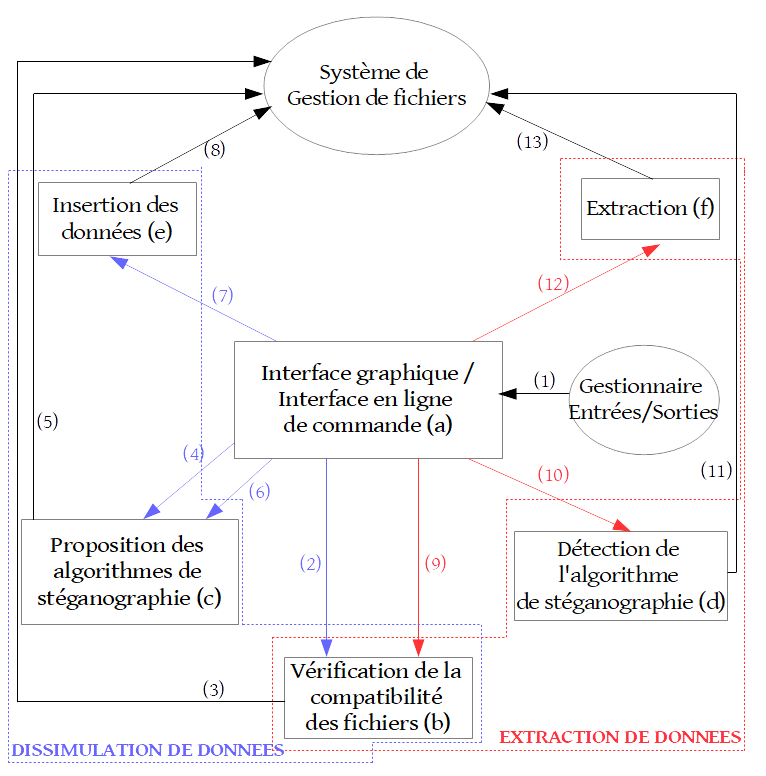
\includegraphics[scale=0.55]{pictures/organigramme.png}
\newpage

L'étude des différentes propriétés de la stéganographie et la stéganalyse 
nous a mené vers cet organigramme. 
Il permet de visualiser les étapes successives de la stéganographie 
(insertion des données), ainsi que celle de la stéganalyse (extraction 
des données). 

Pour la dissimulation de données, il va d'abord y avoir la \textit{Vérification 
de la compatibilité} (b) du fichier hôte, pour savoir si le format est bien 
pris en charge par l'application. 
Il y a ensuite le module \textit{Proposition des algorithmes de stéganographie} 
(c) qui va être utilisé. Un premier appel vers ce module permettra de proposer 
un ou plusieurs algorithmes en fonction du fichier hôte et du fichier à cacher (flèche 4). 
Puis, le deuxième appel permettra à l'utilisateur de choisir l'algorithme 
parmi ceux proposés précedemment (flèche 6). 
La dernière étape consiste en la réelle insertion des données, où les 
données à cacher seront dissimulées dans une copie du fichier hôte (flèche 7). 

Pour l'extraction de données, le module \textit{Vérification de la compatibilité 
des fichiers} permettra, comme pour l'insertion, de vérifier si le format 
du fichier à analyser est bien pris en charge. 
Il y aura ensuite une \textit{Détection de l'algorithme de stéganographie} 
(flèche 10) permettant de trouver la méthode utilisée par l'émetteur pour 
cacher les données. 
Enfin, l'\textit{Extraction} (f) permettra de récupérer les données cachées 
dans le fichier à analyser (flèche 12). 

Tous ces modules et sous-modules seront coordonnées grâce aux interfaces 
graphique et en ligne de commande (a), proposées par StegX. 


\section{Description du fonctionnement}

Pour montrer le fonctionnement de l'application, nous allons proposer un 
exemple pour dissimulation et un autre pour l'extraction, correspondant 
à une communication entre Alice et Bob, surveillée par Oscar. 
Les données sont issues d'une réelle utilisation de StegX. 

\subsection{Prérequis}

On suppose que, lors de l'insertion, l'utilisateur choisit un fichier hôte
vierge : c'est-à-dire que ce dernier n'a pas été utilisé avant pour la 
dissimulation d'un autre fichier. 

De plus, on suppose que, lors de l'extraction, l'utilisateur fournit à 
l'application un fichier contenant des données cachées par StegX. 

Enfin, on fait l'hypothèse que pour les fichiers hôtes et à cacher pour l'insertion 
ainsi que pour les fichiers à analyser pour l'extraction, l'utilisateur a 
les droits d'accès en lecture. 

\subsection{Fonctionnement des modules}

\subsubsection{Fonctionnement du module Vérification de la compatibilité des 
fichiers}

Ce module est commun à l'insertion et l'extraction. Il correspond à la 
recherche détaillée de la nature du fichier hôte. 
Pour cela, il va y avoir une batterie de tests durant lesquels les
signatures des différents formats proposés par l'application vont être recherchées. 
Si l'une d'elle est reconnue, cela signifie qu'il s'agit du format en question. 
A la fin de la batterie de tests, si le format n'a pas été reconnu, 
l'application renvoie une erreur : en effet, elle ne peut pas utiliser ce 
fichier là pour dissimuler ou extraire des données. 

\subsubsection{Fonctionnement de Proposition des algorithmes de stéganographie}

Dans ce module, l'application va lire en détails les particularités du fichier 
hôte. En effet, dans le module précédent, nous avons trouvé le format. Il 
faut maintenant lire le header du fichier pour l'interpréter correctement 
par la suite. Lorsque les données spécifiques du fichier ont été trouvées, 
une batterie de tests sur les différents algorithmes proposés par l'application
permettra de déterminer quels algorithmes sont possibles avec la nature 
du fichier hôte et la taille du fichier à cacher. 
Après cette batterie de tests, la récupération du choix de l'utilisateur 
permettra de déterminer son choix d'algorithme à utiliser lors de l'insertion. 

\subsubsection{Fonctionnement de Détection de l'algorithme de stéganographie}

Ce module correspond à la lecture de la signature StegX. En fonction du 
format du fichier à analyser, le décalage de la lecture de la signature StegX
dans le fichier ne sera pas le même. Cette lecture sera déterminante pour 
découvrir l'algorithme utilisé, le nom du fichier caché et la taille de 
ce dernier. 

\subsubsection{Fonctionnement de Insertion}

Lorsque le fichier à cacher, l'algorithme de stéganographie à utiliser, 
la nature du fichier hôte, le mot de passe (s'il y en a un) et l'emplacement 
du fichier à créer sont connus, il est temps de réaliser la dissimulation. 
Chaque algorithme diffère plus ou moins pour chaque format. 
L'étape commune est le fait que si le fichier à cacher est trop grand, 
l'utilisation du mot de passe permettra de générer (à partir d'une graine), 
une suite de nombres pseudo-aléatoires afin de faire un XOR avec chaque 
octet du fichier à cacher. Si la taille le permet, les octets à cacher 
seront mélangés (grâce au mot de passe) afin de rendre impossible l'extraction 
par une personne inconnue. 

\subsubsection{Fonctionnement de Extraction}

De la même manière que l'insertion, lorsque le nom du fichier caché, la taille 
du fichier caché, l'algorithme, le mot de passe (s'il y en a un) et l'emplacement
du fichier prochainement extrait sont connus, l'extraction peut commencer. 
Le mot de passe permettra de retrouver la même suite de nombres pseudo-aléatoires 
pour XOR avec les octets extraits (si le fichier caché est trop gros). 
Si sa taille le permet, le fichier caché sera créé en remettant dans l'ordre 
les octets extraits. 

\subsection{Description technique de la signature StegX}

La signature StegX est primordiale dans l'insertion puisqu'elle permet au 
destinataire de pouvoir interpréter ce que l'émetteur a voulu lui communiquer. 
Pour cela, cette signature doit avoir plusieurs champs : 
\begin {enumerate}
\item Identificateur de la méthode (1 octet) : cette variable correspond au 
champ \textit{method} de la structure privée \textit{info\_s}. L'octet ne 
peut prendre que deux valeurs possibles : la méthode avec ou sans mot de 
passe. Si l'émetteur choisit un mot de passe, StegX récupèrera ce mot de 
passe pour réaliser l'insertion de façon sécurisée. Le destinataire devra 
choisir le même mot de passe pour extraire les données correctement. 
Si par contre, l'émetteur ne choisit pas de mot de passe, StegX va en choisir 
un au hasard et faire les mêmes manipulations qu'avec un mot de passe. 
Le mot de passe par défaut devra donc être écrit dans la signature afin que 
le destinataire puisse extraire. 
\item Identificateur de l'algorithme (1 octet) : cette variable représente 
l'algorithme utilisé par l'émetteur pour que le récepteur extrait correctement 
les données. 
\item Taille du fichier caché (4 octets) : ce nombre représente en octets 
la taille du fichier caché dans le fichier hôte. Il a une taille maximale 
de $2^{32}$ octets, soit 4 GB. Ce nombre est écrit en little endian. 
\item Taille du nom du fichier caché (1 octet) : cet octet représente le 
nombre de caractères du nom du fichier caché sans compter le caractère de 
fin '$\backslash$0'. Si lors de la dissimulation l'émetteur donne un fichier 
dont le nom est trop long, son nom sera coupé à 255 caractères. 
\item Nom du fichier caché (entre 1 et 255 octets) : représente le nom du 
fichier caché. Ce nom va être XOR avec le mot de passe (par défaut ou choisi
par l'utilisateur) : ainsi, si le récepteur choisit un mot de passe différent, 
il ne pourra même pas connaître le nom du fichier caché. 
\item Mot de passe (64 octets) : représente le mot de passe par défaut choisi 
aléatoirement par l'application. Si la méthode est avec mot de passe, 
ce champ n'existe pas car c'est le destinataire qui doit le connaître et 
non l'application qui doit l'extraire. 
\end{enumerate}

\subsection{Description technique des algorithmes proposés}

% mettre un prerequis disant que soit cest XOR soit cest pur melange

\subsubsection{Algorithme End Of File}

Pour l'insertion des données, cet algorithme consiste à recopier le fichier 
hôte dans le fichier résultat, suivi de la signature, suivi des octets 
représentant le fichier à cacher. Cet algorithme fonctionne car les éditeurs 
des formats pour lesquels l'algorithme est proposé n'interprètent pas les données 
après la fin "officielle" du fichier. 

Pour l'extraction des données, il faut aller à la fin officielle du fichier 
à analyser. A cet endroit précis est écrit la signature StegX. Ainsi, 
les informations sur le fichier caché sont interprétées. Puis, il y a une 
lecture après cette signature, correspondant aux données cachées. 

\subsubsection{Algorithme Least Significant Bit}

Pour l'insertion des données, l'algorithme LSB va modifier les bits de 
poids faible des différents octets des données de l'hôte. Selon la taille des
données à cacher et la taille du fichier hôte, les données cachées pourront 
être dispersées dans les octets de l'hôte. Sinon, on exercera un XOR avec 
la suite pseudo-aléatoire générée à partir du mot de passe. 
Ensuite, quand toutes les données de l'hôte modifiées par LSB ont été écrites 
dans le fichier résultat, la signature StegX est écrite. 

Pour l'extraction des données, la lecture de la fin du fichier permettra de 
lire la signature StegX. Ensuite, les octets de l'hôte seront lues afin d'extraire 
les données cachées. 

\subsubsection{Algorithme Metadata}

Pour chaque format pris en charge par StegX qui propose cet algorithme, 
Metadata diffère. En effet, l'étude approfondie du format du fichier est 
nécessaire pour connaître les endroits du fichier où cacher des données. 

Pour l'insertion, il est nécessaire que la signature StegX soit écrite à 
la fin du fichier afin que l'extraction puisse se dérouler correctement. 

\subsubsection{Algorithme End Of Chunk}

Cet algorithme est uniquement proposé par le format FLV et consiste à 
écrire après les différents chunks du fichier hôte. En effet, lors de 
son interprétation, les chunks non reconnus sont ignorés. C'est donc une 
variante de l'algorithme Metadata car on manipule les données pour que 
les interpréteurs de format FLV les ignorent. 

\subsubsection{Algorithme Junk Chunk}

L'algorithme Junk Chunk est seulement proposé par le format AVI. Il correspond 
à la création d'un chunk Junk. Ce chunk est spécifique car il représente 
un chunk poubelle dans lequel les données ne seront pas interprétées. 

\subsection{Fonctionnement dans un exemple}

\subsubsection{Fonctionnement de l'insertion des données par un exemple}

Alice choisit de dissimuler le message dans une image qu'elle veut envoyer 
à Bob à l'aide de l'interface graphique. 
Tout d'abord, elle choisit les entrées de la dissimulation : le fichier 
à cacher, le fichier hôte ainsi que le chemin du fichier à créer et un mot 
de passe pour augmenter la sécurité de la dissimulation. 
Dans cet exemple, le fichier à cacher est /home/user/Bureau/message.txt 
de taille 2.2 kB ; le fichier hôte est /home/user/Images/photo.bmp 
de taille 21.1 MB ; le chemin du fichier à créer est 
/home/user/Documents/piece\_jointe.bmp ; le mot de passe est "alicebob" 
(communiqué à Bob sur un canal sûr). 

L'interface va appeler le module \textit{Vérification de la compatibilité 
des fichiers}. Le type du fichier hôte sera analysé grâce à la lecture 
de l'entête du fichier : il s'agit d'un fichier BMP non compressé dont les 
pixels sont codés sur 24 bits (8 bits par composantes couleurs). 
Le sous-module \textit{Proposition des algorithmes de stéganographie} va 
remplir la structure spécifique 
\textit{infos.host.file\_info.bmp}, notamment avec le 
\textit{header\_size} égal à $122$ octets, le \textit{data\_size} égal à 
$21085440$ octets, le champ \textit{pixel\_length} égal à $24$ et le champ 
\textit{pixel\_number} égal à $2584 \times 2720 = 7028480$. De cette structure
est déduit les algorithmes proposés (EOF, LSB et Metadata). 
Dans cet exemple, Alice choisit l'algorithme EOF. 

La prochaine étape est celle de l'insertion. Pour la stéganographie EOF, 
StegX va écrire dans /home/user/Documents/piece\_jointe.bmp le fichier hôte. 
Ensuite, la signature StegX est écrite dans lequel on a l'identificateur 
de la méthode (1 octet), l'identificateur de l'algorithme (1 octet), la 
taille du fichier caché noté en little endian (sur 4 octets), la taille du 
nom du fichier caché (1 octet) et le nom du fichier caché XOR avec le mot 
de passe "alicebob" choisi au début. 
Enfin, les données cachées sont également écrites à l'aide du mot de passe
grâce à l'algorithme de protection des données. 

Alice pourra donc envoyer le fichier piece\_jointe.bmp qui aura une taille 
de 21088071 octets soit 21.1 MB sur un canal non sécurisé. 

Oscar, qui espionne les communications entre Bob et Alice, n'aura aucun 
soupçon en voyant piece\_jointe.bmp qui semble être une image comme une 
autre. 

\subsubsection{Fonctionnement de l'extraction des données par un exemple}

Bob reçoit sur le canal non sûr le fichier piece\_jointe.bmp et sait que 
ce fichier contient des données cachées. Pour les extraire, Bob choisit 
d'utiliser StegX avec l'interface en ligne de commande. 

Il tape dans son terminal \textit{stegx -e -o piece\_jointe.bmp -r 
/home/user/Bureau/ -p alicebob} qui signifie que Bob veut extraire les 
données cachées du fichier piece\_jointe.bmp, que le résultat de ces 
données extraites doivent être écrites dans son Bureau et que Bob veut 
extraire les données cachées à l'aide du mot de passe "alicebob"

Tout d'abord, le module \textit{Vérification de la compatibilité des 
fichiers} va analyser le type de piece\_jointe.bmp. Il s'agira bien du 
format BMP non compressé. 

Ensuite, le module \textit{Détection de l'algorithme de stéganographie}
permettra de remplir la structure spécifique de \textit{infos.host.file\_info.bmp}
et déduira les mêmes champs que Alice lors de l'insertion. En effet, 
il va y avoir une lecture approfondie du fichier. Ensuite, la signature 
StegX, qui a été écrite lors de l'insertion, sera lue pour en déduire 
le nom du fichier caché, l'algorithme et la taille du fichier caché. 

Enfin, le module \textit{Extraction}, appelé par l'interface, va réaliser 
l'extraction. Ici, les données cachées seront extraites grâce au mot de passe 
"alicebob" choisi par Alice lors de l'insertion et nécessaire pour l'extraction 
effectuée par Bob. 
Les données cachées extraites seront écrites dans le fichier
/user/home/Bureau/message.txt. Bob pourra ainsi lire le message de Alice 
contenu dans le fichier message.txt. 

\section{Description des points délicats de la programmation}

\subsection{Lecture et écriture de fichiers \& endianness}

La première difficulté est arrivée lors de l'implémentation du module 
\textit{Vérification de la compatibilité des fichiers}. En effet, il fallait 
lire la signature des fichiers hôtes pour l'insertion et l'extraction. 

Nous ne comprenions pas pourquoi sur certains formats le little-endian 
était utilisé et sur d'autres il fallait utilisé le big-endian. 
De plus, il fallait également convertir les octets lus dans l'endian de la 
machine de l'utilisateur. L'équipe de conception a fait des recherches à 
propos des processeurs little/big endian et les processeurs big-endian sont 
des processeurs pour les systèmes embarqués. De ce fait, il fallait lire 
les données des fichiers et les convertir en little endian. 

Nous avons donc trouvé une solution : la création de fonctions de 
conversion entre les deux endianness. L'équipe StegX pouvait utiliser la 
librairie \textit{endian.h} mais l'application est multi-plateforme (Linux 
et Windows) et cette librairie n'était pas standard. Le meilleur moyen était 
donc de reproduire ces fonctions de conversion pour l'application 
\label{endian}. 

\subsection{Etude des différents formats \& algorithme Metadata}

La deuxième difficulté rencontrée est celle de l'implémentation de 
l'algorithme Metadata. La particularité de cet algorithme est le fait 
qu'elle dépend du format du fichier hôte. C'est d'ailleurs avec la fonction 
\textit{fill\_host\_info} que la structure-union était remplie et qu'on 
distinguait les éléments importants du format en question.  
Il faut donc étudier avec précision la nature des éléments qui composent
ce format.  

\subsection{Format MP3}

Le format MP3 est sans nul doute le format le plus compliqué de ceux
que l'équipe StegX s'est occupé. En effet, il s'agit d'un format compressé 
utilisant des algorithmes de compression divers et complexes. 
Pour ce format, il a fallu que le binôme composé de Pierre Ayoub et Damien 
Delaunay, chargé de réaliser l'insertion et l'extraction des formats audio, 
décordique les spécifications précises de plusieurs versions du format 
(MPEG 1 Layer III, MPEG 2 Layer III), et de plusieurs versions de formats 
de métadonnée (ID3 version 1 et ID3 version 2). 
Une fois cela fait, il a fallu récupérer plusieurs fichiers échantillons 
correspondant aux différents formats et versions afin de les analyser en 
hexadécimal et en faire la lecture pour en comprendre le mécanisme. Ces 
opérations ont été longues et pointilleuses et aucun algorithme ne pourra 
être proposé dans la version de StegX rendue pour le 25 mai. 

Il était peut-être trop ambicieux pour StegX de proposer un format aussi 
complexe. 

\section{Changements mineurs des spécifications}

\subsection{Changements de noms}

Le nom de la variable globale \textit{algo\_e* proposition} qui va sauvegarder 
les algorithmes possibles lors de l'insertion a changé et devient 
\textit{stegx\_propos\_algos}. 

Les deux noms de fonctions \textit{int insert(info\_s* infos)} et 
\textit{int extract(info\_s* infos, char* res\_path)} deviennent 
\textit{stegx\_insert} et \textit{stegx\_extract}. 

\subsection{Ajouts de fonctions pour éviter la répétition de code}

Pour l'algorithme de protection des données qui consiste à mélanger/remettre
en ordre les octets du fichier caché, l'équipe de conception a créé plusieurs 
fonctions qui sont utilisés dans tous les algorithmes proposés par StegX. 
Il fallait donc créer ces fonctions afin d'éviter une répétition de code :
 
\begin{lstlisting}[language=c]
unsigned int create_seed (const char* passwd)
\end{lstlisting}

Elle consiste à créer à partir du mot de passe une graine permettant de 
générer une suite pseudo-aléatoire. Cette suite sera utilisée pour le 
mélange et le XOR des octets à cacher. 
\newline
\underline{Entrée :}
\begin{itemize}
\item \textit{*passwd :} Mot de passe utilisé pour créer la graine. 
\end{itemize}
\underline{Sortie :} 
\begin{itemize}
\item \textit{unsigned int :} renvoie la graine de la suite pseudo aléatoire.
Elle sera le paramètre de la fonction \textit{srand} pour initialiser cette 
suite.   
\newline 
\end{itemize}

\begin{lstlisting}[language=c]
int protect_data (uint8_t* tab, uint32_t hidden_length, const char* passwd, 
	mode_e mode)
int protect_data_lsb(uint8_t * pixels, uint32_t pixels_length, uint8_t * data, 
	uint32_t data_length, char *passwd, mode_e mode)
\end{lstlisting}

La première fonction fait le mélange ou réarrange les octets à cacher selon 
l'algorithme de protection des données. Lors de l'insertion, les octets seront 
mélangés et lors de l'extraction, les octets seront remis dans le bon ordre. 
La première fonction sera utilisée par tous les algorithmes de stéganographie 
d'insertion et extraction exceptée l'algorithme LSB.  
De la même manière, pour enlever la répétition de code pour l'algorithme 
LSB lors de la protection des données, la deuxième fonction permet de 
dissimuler/extraire les octets cachés dans des pixels (image) et des 
échantillons (audio) différents. Elle sera utilisée uniquement pour les 
algorithmes d'insertion et d'extraction LSB. 

\underline{Entrées :}
\begin{itemize}
\item \textit{*tab (1) :} Tableau d'octets à réarranger. 
\item \textit{hidden\_length (1) :} Taille du tableau tab.
\item \textit{*pixels (2) :} Tableau d'octets du fichier hôte. 
\item \textit{pixels\_length (2) :} Taille du tableau pixels. 
\item \textit{*data (2) :} Tableau d'octets à cacher. 
\item \textit{data\_length (2) :} Taille du tableau data. 
\item \textit{*passwd :} Mot de passe utilisé pour générer la graine. 
\item \textit{mode :} Mode qui peut être soit STEGX\_MODE\_INSERT ou 
STEGX\_MODE\_EXTRACT. 
\end{itemize}
\underline{Sortie :} 
\begin{itemize}
\item \textit{int :} renvoie 1 si il y a une erreur détectée dans cette 
fonction et 0 si tout se passe bien.  
\newline 
\end{itemize}

Pour l'algorithme EOF, lors de l'insertion et l'extraction, l'utilisation 
du XOR et de l'algorithme de protection des données étaient nécessaires. 
L'équipe StegX a donc créé deux fonctions pour éviter la répétition de code : 

\begin{lstlisting}[language=c]
int data_xor_write_file (FILE* src, FILE* res, const char* passwd)
\end{lstlisting}

Elle va écrire les données XORés avec la suite générée par le mot de passe. 
\newline
\underline{Entrées :}
\begin{itemize}
\item \textit{* src :} Fichier où lire les données à XORé. 
\item \textit{* res :} Fichier où écrire les données à XORé. 
\item \textit{*passwd :} Mot de passe utilisé pour créer la graine. 
\end{itemize}
\underline{Sortie :} 
\begin{itemize}
\item \textit{int :} renvoie 1 si il y a une erreur détectée dans cette 
fonction et 0 si tout se passe bien. 
\newline 
\end{itemize}

\begin{lstlisting}[language=c]
int data_scramble_write (FILE* src, FILE* res, const char* passwd, 
	const uint32_t len, const mode_e m)
\end{lstlisting}

Elle va écrire les données mélangées ou remises en ordre grâce au mot de 
passe. 
\newline
\underline{Entrées :}
\begin{itemize}
\item \textit{* src :} Fichier où lire les données à XORé. 
\item \textit{* res :} Fichier où écrire les données à XORé. 
\item \textit{*passwd :} Mot de passe utilisé pour créer la graine. 
\item \textit{len :} Longueur des données à cacher/cachées. 
\item \textit{m :} Mode d'utilisation (STEGX\_MODE\_INSERT ou STEGX\_MODE\_EXTRACT). 
\end{itemize}
\underline{Sortie :} 
\begin{itemize}
\item \textit{int :} renvoie 1 si il y a une erreur détectée dans cette 
fonction et 0 si tout se passe bien. 
\newline 
\end{itemize}

Pour éviter une répétition de code pour l'algorithme EOF où il faut se 
déplacer jusqu'à la fin de la signature pour lire/écrire les données cachées
 ou à cacher, une nouvelle fonction a été créée : 

\begin{lstlisting}[language=c]
int sig_fseek(FILE* f, char * h, method_e m)
\end{lstlisting}
\underline{Entrées :}
\begin{itemize}
\item \textit{* f :} Fichier où faire le saut. 
\item \textit{* h :} Nom du fichier caché écrit dans la signature. 
\item \textit{m :} Méthode avec ou sans mot de passe par défaut. 
\end{itemize}
\underline{Sortie :} 
\begin{itemize}
\item \textit{int :} renvoie la valeur du fseek lors du saut. 
\newline 
\end{itemize}

\subsection{Ajouts pour l'optimisation}

Tout d'abord, par soucis d'optimisation afin d'éviter à un futur développeur 
de se tromper lors de mises à jour de StegX, nous avons rajouté un champ 
\textit{STEGX\_NB\_ALGO} \underline{mis en dernier} dans l'énumération \textit{algo\_e}. 
Cet ajout permet de connaître facilement le nombre d'algorithmes implémentés 
utile surtout dans le module \textit{Proposition des algorithmes de stéganographie}. 
\newline

Pour permettre un débuggage précis, l'équipe StegX a créé une énumération qui
recense toutes les erreurs possibles dans StegX : \textit{enum err\_code}. 
Ainsi, si il y a une erreur en plein milieu d'une extraction, l'utilisateur 
pourra identifier le problème très facilement. Vu que cette gestion d'erreurs 
est effectuée par les deux interfaces, il fallait donc la créer dans les 
fichiers sources de la librairie et non dans chaque interface. De plus, 
une fonction \textit{void err\_print(const enum err\_code err)} permet aux 
interfaces de montrer à l'utilisateur s'il y a un problème. 
\newline

La taille d'un type \textit{int} peut dépendre en fonction de l'architecture
de la machine de l'utilisateur : en effet, il peut être égal à 2 ou à 4 octets. 
De ce fait, pour uniformiser cette nuance, nous avons changé le type 
\textit{int hidden\_length} de \textit{struct info} par \textit{uint32\_t}. 
Ainsi, cela permet d'avoir 4 octets pour toutes les machines. 
\newline 

Comme vu précédemment dans le paragraphe \ref{endian}, il a fallu créer 
des fonctions de conversion d'entiers d'un endian à un autre : 

\begin{lstlisting}[language=c]
uint32_t stegx_htobe32(uint32_t nb)
uint32_t stegx_be32toh(uint32_t nb)
\end{lstlisting}

La première fonction permet de convertir de passer de \textit{nb} little 
endian en big endian. 
La deuxième fonction consiste à passer \textit{nb} de big endian en 
little endian. 

\section{Comparaison estimation - implémentation}

\small
\hspace{-1cm}
\begin{tabular}{|c|c|c|c|}
  \hline
  \textbf{Module de l'application} & \textbf{Coût en nombre de lignes} & \textbf{Coût en temps} & \textbf{Personnel(s) en charge} \\
  \hline
    Interface en ligne & Estimation : 200 lignes & Estimation : 30 heures & BASKEVITCH Claire \& \\ 
    de commande & Implémentation : 200 lignes & Implémentation : 30 heures & BESSAC Tristan \\
  \hline
  Interface & Estimation : 400 lignes & Estimation : 30 heures & AYOUB Pierre \& \\
  graphique & Implémentation : 400 lignes & Implémentation : 30 heures & DELAUNAY Damien \\
  \hline
  Vérification de la & Estimation : 300 lignes & Estimation : 30 heures & CAUMES Clément \& \\
   compatibilité des fichiers & Implémentation : 150 lignes & Implémentation : 15 heures & DOUDOUH Yassin \\
  \hline
    Proposition des algos & Estimation : 100 lignes & Estimation : 15 heures & CAUMES Clément \& \\
   de stéganographie & Implémentation : 210 lignes & Implémentation : 30 heures & DOUDOUH Yassin \\
  \hline
    Détection de l'algo & Estimation : 100 lignes & Estimation : 15 heures & AYOUB Pierre \& \\
   de stéganographie & Implémentation : 60 lignes & Implémentation : 15 heures & DELAUNAY Damien \\
  \hline
  Dissimulation \& Extraction & Estimation : 250 lignes & Estimation : 40 heures & CAUMES Clément \& \\
   fichiers images & Implémentation : X lignes & Implémentation : X heures & DOUDOUH Yassin \\
  \hline
  Dissimulation \& Extraction & Estimation : 250 lignes & Estimation : 40 heures & AYOUB Pierre \& \\
   fichiers audios & Implémentation : X lignes & Implémentation : X heures & DELAUNAY Damien \\
     \hline
  Dissimulation \& Extraction & Estimation : 250 lignes & Estimation : 40 heures & BASKEVITCH Claire \& \\
   fichiers vidéos & Implémentation : X lignes & Implémentation : X heures & BESSAC Tristan \\
  \hline
\end{tabular}
\normalsize
\vspace{0.5cm}

En comparant l'estimation du nombre de lignes établie dans le cahier des 
charges et le nombre de lignes codées lors de l'implémentation, on remarque 
plusieurs détails : 

\begin{itemize}
\item L'estimation pour les deux interfaces ont été justes malgré le fait 
que l'équipe StegX ne connaissait pas GTK+. Elle a dû faire une estimation 
globale qui a été finalement juste. 
\item On peut voir que le module \textit{Vérification de la compatibilité}
est 2 fois plus long que l'estimation et que le module \textit{Proposition 
des algorithmes} est 2 fois plus court que l'estimation. Cela s'explique 
par le fait que, lors de l'élaboration du cahier des charges l'équipe StegX
pensait que trouver les détails nécessaires à l'insertion (rôle de la fonction 
\textit{fill\_host\_info}) devait se faire dans le module \textit{Proposition 
des algorithmes} et non dans celui-ci.  
\end{itemize}

\section{Bilan technique du produit et Améliorations pour les versions futures}

Le produit StegX répond bien aux objectifs : faire de la stéganographie 
et de la stéganalyse sur des fichiers de type image, audio et vidéo en 
utilisant plusieurs algorithmes (LSB, EOF, Metadata). 
Par ailleurs, StegX propose bien 2 interfaces : une en ligne de commande 
et une autre graphique. 
Avoir choisi le langage C a été le meilleur choix car ce langage nous a 
permis de manipuler facilement les données binaires des fichiers en entrée. 

En plus de répondre aux objectifs, l'équipe de conception s'est efforcée 
à répondre aux nombreux besoins du client, qui doit rester la personne la 
satisfaite du produit. 

En ce qui concerne les algorithmes proposés par StegX en fonction des 
formats pris en charge, voici le bilan de ce que propose l'application : 
\newline

\begin{tabular}{|l|c|c|c|c|c|}
  \hline
  \multirow{2}*{\textbf{Format pris en charge par l'application}} & \multicolumn{5}{c|}{\textbf{Algorithmes proposés}} \\
   \cline{2-6}
    & \textbf{LSB} & \textbf{EOF} & \textbf{Metadata} 
    &\textbf{EOC} & \textbf{Junk Chunk} \\
  \hline
  \textbf{BMP} (Clément Caumes \& Yassin Doudouh) & \textbf{\checkmark} & \textbf{\checkmark} & \textbf{\checkmark} &  & \\
  \hline      
  \textbf{PNG} (Clément Caumes \& Yassin Doudouh) &  & \textbf{\checkmark} & \textbf{\checkmark} & & \\
  \hline
  \textbf{WAV} (Pierre Ayoub \& Damien Delaunay) & \textbf{\checkmark} & \textbf{\checkmark} & & & \\
  \hline 
  \textbf{AVI} (Claire Baskevitch \& Tristan Bessac) & & & & & \textbf{\checkmark}\\
  \hline
  \textbf{FLV} (Claire Baskevitch \& Tristan Bessac) & & \textbf{\checkmark} & & \textbf{\checkmark} & \\
  \hline
\end{tabular}
\vspace{0.5cm}

Concernant les améliorations à apporter pour l'application, cela aurait été 
intéressant, pour les fichiers hôte (pour l'insertion et pour l'extraction)
dont l'utilisateur n'a pas les droits de lecture, de modifier ces droits. 
De plus, l'avantage de ce produit est le fait qu'il peut être constamment 
en amélioration du fait que l'on peut gérer encore plus de formats et 
sûrement d'autres algorithmes de stéganographie. 

\section{Conclusion sur l'organisation interne au sein du projet}

Durant le semestre 6 de la dernière année de licence informatique à Versailles, 
l'équipe StegX s'est réunie pour créer une application en rapport à la 
cryptographie. 
De ce fait, tous les membres de l'équipe de conception se sont efforcés à
travailler de façon professionnelle et ordonnée. En effet, ils leur tenaient 
à coeur de mettre en application toute la méthodologie informatique acquise 
durant la licence. 
Par ailleurs, en raison de la grande charge de travail, il a fallu, dès le 
début du projet, diviser la conception selon les trois différents types 
dont StegX doit se charger (image, audio et vidéo). 
Cette division de charge de travail impliquait que chacun devait réaliser 
une partie de la conception. 

Enfin, nous n'avions pas de chef de projet. Cette décision nous a été très 
favorable du fait que chacun a eu la maturité de comprendre les enjeux de 
ce grand projet. En effet, ces enjeux étaient grands et c'est pour cela 
que le projet IN608 est la matière la plus travaillée du semestre. C'était 
d'ailleurs le projet préféré de la licence car il était de très grande 
envergure et dont l'équipe a proposé le sujet. 

Damien Delaunay a été absent durant plusieurs entretiens avec le client 
en raison de graves problèmes familiaux. Cela ne l'a pas empêché de travailler 
durant le semestre lors des réunions et les conférences entre les membres 
de l'équipe StegX. 

\end{document}
